% TikZ diagram for black-box safety validation problem formulation.
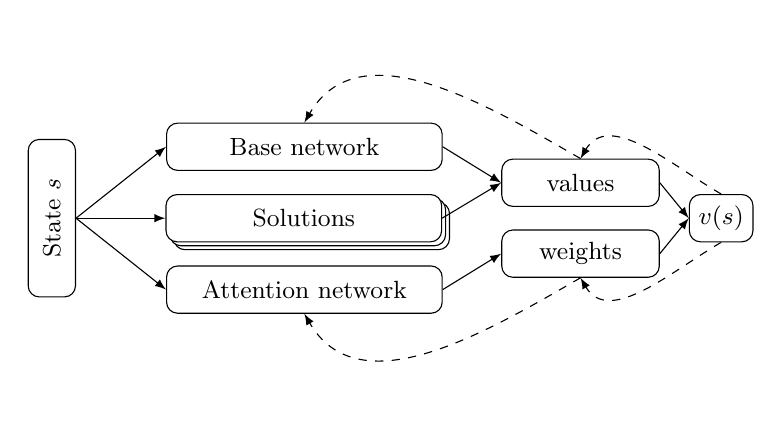
\begin{tikzpicture}
    \tikzstyle{every node}=[font=\small, align=center]
    \tikzset{
        n/.style={draw, rounded corners, minimum height=0.6cm, minimum width = 2cm},
        n2/.style={n, minimum width=3.5cm}
        }
    
    %state 
    \node (state) [n, rotate=90] {\small State $s$};
    
    %base network
    \node (base) [n2, above right of=state, xshift=2.5cm, yshift = 0.2cm] {Base network};
    
    %Solutions
    \node (solutionsback1) [n2, right of=state, xshift=2.3cm, yshift=-0.1cm] {};
    \node (solutionsback2) [n2, fill=white, right of=state, xshift=2.25cm, yshift=-0.05cm] {};
    \node (solutions) [n2, fill=white, right of=state, xshift=2.2cm] {Solutions};
    
    %weights
    \node (attn) [n2, below right of=state, xshift=2.5cm, yshift=-0.2cm] {Attention network};
    

    \node (values) [n, below right of=base, xshift=2.8cm, yshift = 0.25cm] {values};
    
     \node (weights) [n, above right of=attn, xshift=2.8cm, yshift = -0.25cm] {weights};
     
     \node (pfail) [n, minimum width = 0.5cm, right of=state, xshift=7.5cm] {$v(s)$};
    

    \draw[-latex] (state.south) -- (base.west);
    \draw[-latex] (state.south) -- (solutions.west);
    \draw[-latex] (state.south) -- (attn.west);
    
    \draw[-latex] (base.east) -- (values.west);
    \draw[-latex] (solutions.east) -- (values.west);
    \draw[-latex] (attn.east) -- (weights.west);
    
    \draw[-latex] (weights.east) -- (pfail.west);
    \draw[-latex] (values.east) -- (pfail.west);
    
    
    % backprop
    
    \draw [dashed, -latex] (weights.south) to [out=-150,in=-60] (attn.south);
    \draw [dashed, -latex] (pfail.south) to [out=-150,in=-60] (weights.south);
    \draw [dashed, -latex] (values.north) to [out=150,in=60] (base.north);
    \draw [dashed, -latex] (pfail.north) to [out=150,in=60] (values.north);
\end{tikzpicture}